\documentclass[conference]{IEEEtran}
\usepackage[ruled,vlined]{algorithm2e}
\usepackage{amsmath}
\usepackage[english]{babel} %localisation
\usepackage{caption,subcaption} %supposedly incompatible with Springer and IOP, IEEETran and ACM SIG
\usepackage{cite} %nice citations, e.g. [1--5]
\usepackage{fixltx2e} %fix latex bugs
\usepackage{graphicx}
\PassOptionsToPackage{hyphens}{url}\usepackage{hyperref} %clickable URLS
\usepackage[htt]{hyphenat} %hyphenate \texttt
\usepackage{microtype} %makes text pretty; also condenses
\usepackage{multirow} %multiple rows in tables
\usepackage{siunitx,textcomp} %\SI{value}{unit}, \si{unit}; textcomp for microtype compatibility
%\usepackage [caption=false]{subfig} %if caption/subcaption not available
% \usepackage{tikz,pgfplots} %drawings and plots
\usepackage[siunitx]{circuitikz} %circuit figures
\usepackage[T1]{fontenc} %ensure proper hyphenation and treatment of math in sentences
\usepackage{booktabs}
\bibliographystyle{IEEEtran}

\usepackage{tikz}
\usetikzlibrary{shapes}
\usepackage{verbatim}
\usepackage{listings}
\begin{document}
\lstset{defaultdialect=[x86]{Assembler}}

% paper title
% can use linebreaks \\ within to get better formatting as desired
\title{Side Channel Analysis of an Embedded/Hardware Crypto Device}

% author names and affiliations
% use a multiple column layout for up to three different
% affiliations
\author{\IEEEauthorblockN{Dallin Marshall, Sam Mitchell, and Nathanael Weidler}
\IEEEauthorblockA{Deptartment of Electrical and Computer Engineering\\
Utah Stat University\\
Logan, Utah 84322\\
e-mail: geekbott@gmail.com, samuel.alan.mitchell@gmail.com, NWeidler@gmail.com}
}

% make the title area
\maketitle


\begin{abstract}
%\boldmath
% Summarize project and results (executive summary).
%
This paper describes the design and implementation of a physically unclonable function (PUF). 

 
\end{abstract}

\begin{IEEEkeywords}
Physically unclonable Function, Device Authentication.
\end{IEEEkeywords}

\section{Introduction}
	A physically unclonable function (PUF) is one method of testing user authentication. The server sends a challenge to a device, and the device responds using the output to the PUF; this is called a challenge response pair. If the PUF is truly unclonable, this authentication method is effectively secure. 

	The analysis of PUFs in authentication relies on 2 characteristics of the PUF: the variation between devices, $\mu_{intra}$, and the reliability of the device to reproduce the same bitstream given a challenge, $\mu_{inter}$. 


\subsection{Related works}

	There are various types of PUFs that can be implemented on an FPGA \cite{VanHerrewege2015}. 

	\cite{VanHerrewege2015} 
	Types of memory-based PUFs.
		\begin{itemize}
			\item SRAM 
			\item Latch (Butterfly) 	\cite{Kumar2008}
			\item Flip-flop \cite{Maes2008,Leest2010}
			\item Buskeeper \cite{Simons2012}
		\end{itemize}

	There are 3 main purposes of PUFs, 
\subsection{Structure of paper}
	The organization is as follows: in Section \ref{sec::des_impl}, the development of the PUF is presented.  In Section \ref{sec::expr} the experimental test setup for the capturing of the challenge response pairs is described. Section \ref{sec::analysis} contains the analysis of the data. Conclusions are detailed in Section \ref{sec::conclusion}. 


\section{Design} \label{sec::des_impl}
	The butterfly PUF consists of wiring 2 NAND gates together in positive feedback mode, as shown in Figure \ref{fig:bfly}. Upon excitation, the gates are put into a race condition until the voltage level converges (less than 1 second). The butterfly should result in a consistent output for each device it's implemented on, while the output of the devices have low correlation. When implemented on a Spartan IV, the majority of the butterfly PUFs gave consistent but unique output, but the logic of 12\% never converges to one voltage. 
		\begin{figure}[tbph]
			\centering
			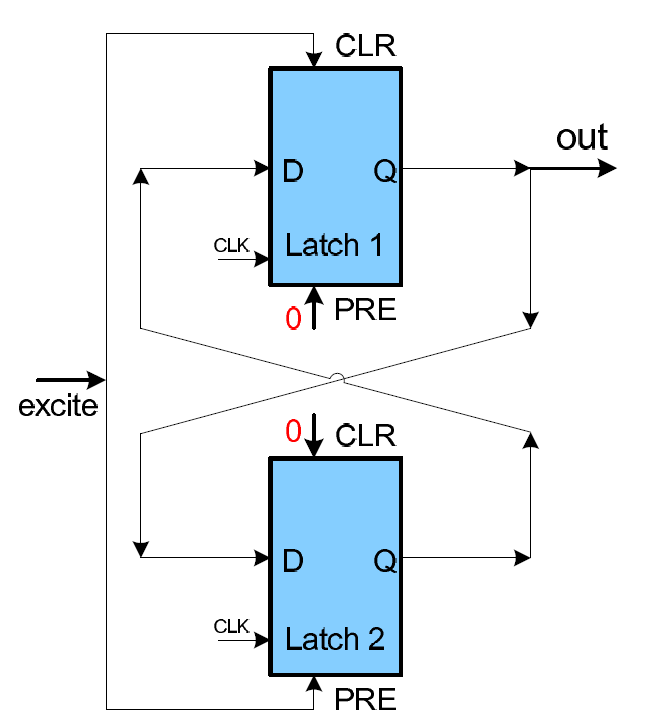
\includegraphics[width=0.3\textwidth]{bfly.png}
			\caption{Butterfly PUF: Cross-coupled latches.}\label{fig:bfly}
		\end{figure}

	This paper utilizes a modified butterfly PUF that accepts an input. The excite signal is used as a switching signal through negation, as shown in Figure \ref{fig:bfly2}. This allows the PUF to accept an input, which results in 2 potential random outputs. Testing showed that some PUFs would consistently toggle, some would consistently remain 1 value, and some weren't consistent, which is consistent with the 12\% of the standard butterfly PUF that wouldn't converge. This PUF is very compact, requiring only 0.03\% of the FPGA space. 
		\begin{figure}[tbph]
			\centering
			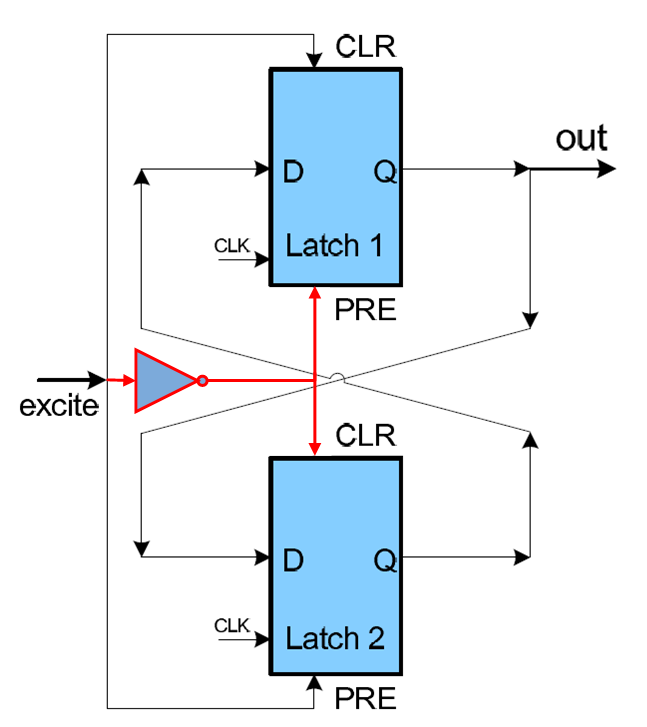
\includegraphics[width=0.3\textwidth]{bfly2.png}
			\caption{Modified-butterfly PUF: Cross-coupled latches are modifiable.}\label{fig:bfly2}
		\end{figure}
		

	\subsection{Butterfly in authentication}
		An authentication device accepts a challenge sequence and sends back a device-specific response. We designed a modified-butterfly PUF authentication device that accepts a 64-bit key input and responds with a 64-bit key. 

		The device is a 64 by 64 grid of modified-butterfly PUFs. Each column uses an XOR gate to accept 1 bit of the 64-bit key; column 1 accepts bit 1, the output of column 1 is XORed with bit 2 and fed to column 2. The row order corresponds with the response bits; row 1 produces bit 1. 

		This design is valid because each bit of the key can alter the response up to 50\%, which means that the corresponding response bit can only be predicted with 50\% accuracy. Each row has a unique string of PUFs, so each response bit will be random to the other bits. 

		A simple verification was performed on this system by implementing 1 row of our modified-butterfly authenticator PUF. Unique keys successfully produced unique responses, but the responses were consistent only 83\% of the time. Without error correction coding, the system will never correctly produce the correct response (0.0064\% likelihood). The modified-butterfly PUF was discarded for authentication applications. 

	\subsection{Butterfly in TRNG}
		TRNG requires random processes to extract numbers from. Both versions of the butterfly PUF produce a race condition before converging to one value. This race condition will quickly settle unless perturbed. 

		Two modified-butterfly PUFs are wired together to induce race conditions in each PUF. This is done by connecting the output of a modified-butterfly PUF to the input of another modified-butterfly PUF, and vice versa. The output of one of the PUFs is sampled periodically (at the communication rate) to produce a stream of random bits. 
		
\section{Experimental Setup} \label{sec::expr}
	
	

\section{Data Analysis}\label{sec::analysis} 

\section{Results}\label{res}

\section{Conclusion}\label{sec::conclusion} 


\nocite{*}
\bibliography{bibpuf}
% that's all folks




\end{document}






